\documentclass[11pt,a4paper]{article}
\usepackage[margin=2.4cm]{geometry}
\usepackage{tikz}
\usetikzlibrary{arrows.meta,positioning,fit,backgrounds,calc}
\usepackage{amsmath,amssymb}
\usepackage{booktabs}
\usepackage[colorlinks=true,linkcolor=black,urlcolor=blue]{hyperref}
\usepackage{parskip}

\definecolor{blind}{RGB}{31,99,163}
\definecolor{market}{RGB}{176,94,24}
\definecolor{joint}{RGB}{38,120,74}
\definecolor{soft}{RGB}{240,240,240}

\tikzset{
  box/.style={draw,rounded corners=2pt,align=center,inner sep=5pt,font=\small},
  blindbox/.style={box,draw=blind,fill=blind!6},
  marketbox/.style={box,draw=market,fill=market!6},
  jointbox/.style={box,draw=joint,fill=joint!8},
  flow/.style={-{Stealth[length=2.5mm]},thick,draw=black!65},
  lab/.style={font=\scriptsize\itshape,inner sep=1.5pt,fill=white},
}

\title{\vspace{-1.5cm}How the pipeline works}
\author{Selective betting with shrinkage}
\date{23 September 2026}

\begin{document}
\maketitle
\vspace{-0.6cm}

\section*{The idea in one paragraph}

A model picks the matches where it disagrees most with the bookmaker. Those are
also the matches where the model is most likely to be wrong, because a large
disagreement is usually a large error rather than a large insight. So the act of
picking selects your own mistakes. The proposed fix is to pull the model's
estimate part of the way toward the market price \emph{before} picking anything.
How far to pull is a single number, $w$, fitted from data.

\section*{The whole pipeline}

Everything the model does is on the left, in blue. Everything the market
contributes is on the right, in orange. They meet once, at the blend.

\begin{center}
\scalebox{0.88}{
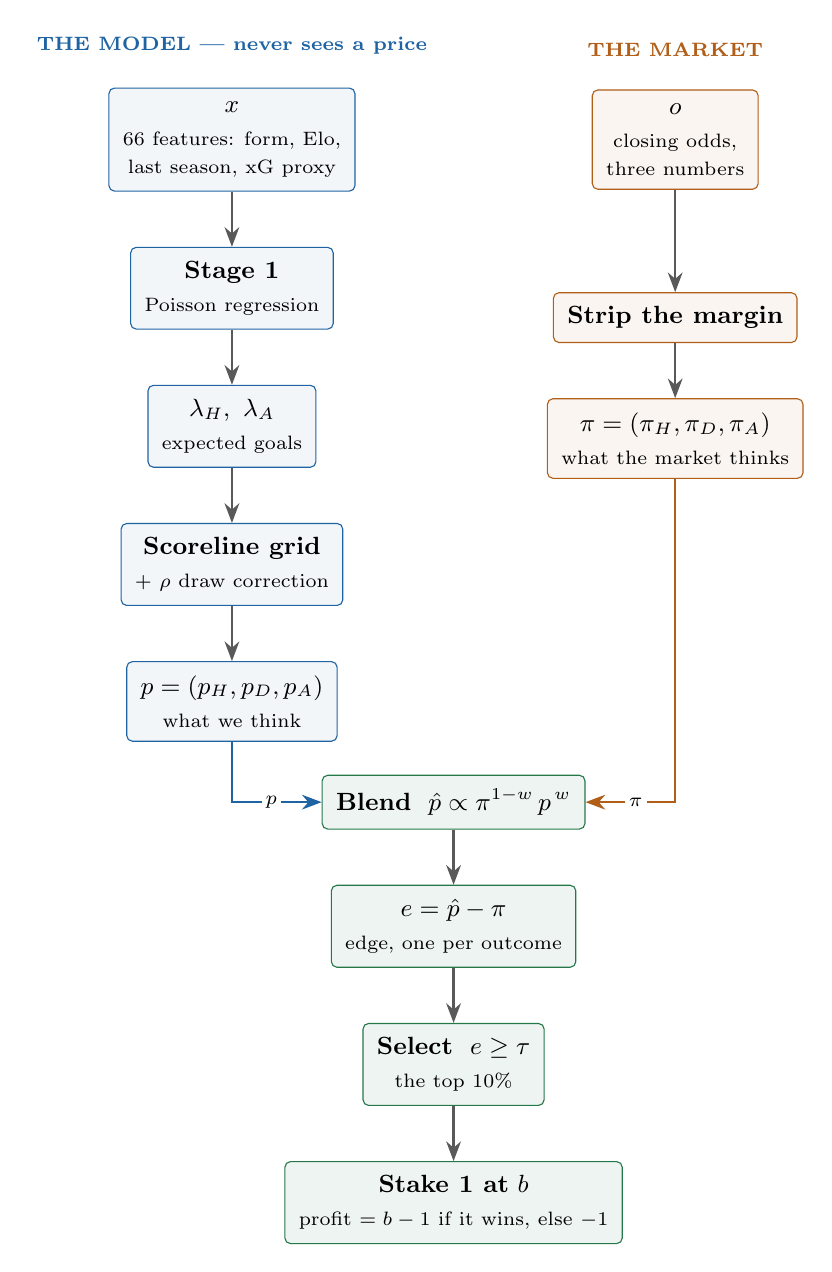
\begin{tikzpicture}[node distance=7mm and 16mm]

\node[blindbox] (x) {$x$\\[1pt]\scriptsize 66 features: form, Elo,\\[-1pt]\scriptsize last season, xG proxy};
\node[blindbox,below=of x] (s1) {\textbf{Stage 1}\\[1pt]\scriptsize Poisson regression};
\node[blindbox,below=of s1] (lam) {$\lambda_H,\ \lambda_A$\\[1pt]\scriptsize expected goals};
\node[blindbox,below=of lam] (grid) {\textbf{Scoreline grid}\\[1pt]\scriptsize $+\ \rho$ draw correction};
\node[blindbox,below=of grid] (p) {$p=(p_H,p_D,p_A)$\\[1pt]\scriptsize what we think};

\node[marketbox,right=30mm of x] (o) {$o$\\[1pt]\scriptsize closing odds,\\[-1pt]\scriptsize three numbers};
\node[marketbox,below=13mm of o] (devig) {\textbf{Strip the margin}};
\node[marketbox,below=of devig] (pi) {$\pi=(\pi_H,\pi_D,\pi_A)$\\[1pt]\scriptsize what the market thinks};

\node[font=\scriptsize\bfseries,blind,above=3mm of x] {THE MODEL --- never sees a price};
\node[font=\scriptsize\bfseries,market,above=3mm of o] {THE MARKET};

\node[jointbox,below=26mm of $(p)!0.5!(pi)$] (blend) {\textbf{Blend}\ \ $\hat p \propto \pi^{1-w}\,p^{\,w}$};
\node[jointbox,below=of blend] (edge) {$e=\hat p-\pi$\\[1pt]\scriptsize edge, one per outcome};
\node[jointbox,below=of edge] (sel) {\textbf{Select}\ \ $e\ge\tau$\\[1pt]\scriptsize the top 10\%};
\node[jointbox,below=of sel] (bet) {\textbf{Stake 1 at} $b$\\[1pt]\scriptsize profit $=b-1$ if it wins, else $-1$};

\draw[flow] (x) -- (s1);
\draw[flow] (s1) -- (lam);
\draw[flow] (lam) -- (grid);
\draw[flow] (grid) -- (p);
\draw[flow] (o) -- (devig);
\draw[flow] (devig) -- (pi);
\draw[flow,draw=blind] (p.south) |- node[lab,pos=0.72]{$p$} (blend.west);
\draw[flow,draw=market] (pi.south) |- node[lab,pos=0.72]{$\pi$} (blend.east);
\draw[flow] (blend) -- (edge);
\draw[flow] (edge) -- (sel);
\draw[flow] (sel) -- (bet);
\end{tikzpicture}}
\end{center}

The blue column never sees a price. That is the whole reason the method can be
tested: if stage 1 had the market among its inputs it would simply copy it, and
pulling it toward the market afterwards would correct nothing.

\section*{Every symbol}

\begin{center}
\begin{tabular}{@{}llll@{}}
\toprule
\textbf{Symbol} & \textbf{What it is} & \textbf{Produced by} & \textbf{Learned?}\\
\midrule
$x$ & 66 market-blind features & the \texttt{build/} scripts & --\\
$\lambda_H,\lambda_A$ & expected goals, each side & stage 1 & \textbf{yes}\\
$\rho$ & low-score draw correction & held-out fit, per league & \textbf{yes}\\
$p$ & model probabilities & scoreline grid & no, arithmetic\\
$o$ & closing average odds & the odds file & --\\
$\pi$ & market probabilities & de-vigging $o$ & no, arithmetic\\
$w$ & shrinkage weight & fitted by log loss & \textbf{yes}\\
$\hat p$ & corrected probabilities & the blend & no, arithmetic\\
$e$ & edge, $\hat p - \pi$ & subtraction & no\\
$\tau$ & selection threshold & 90th percentile of $e$ & from past seasons\\
$b$ & best closing odds & the odds file & --\\
\bottomrule
\end{tabular}
\end{center}

Only three things are learned: $\lambda$, $\rho$ and $w$. Everything else is
arithmetic or a look-up. The method has very few free parameters, deliberately.

\newpage
\section*{Stage 1: from features to a scoreline}

Stage 1 does not predict who wins. It predicts how the match is played, as two
expected-goal counts, then the outcome probabilities are computed from those.

Given $\lambda_H$ and $\lambda_A$, the chance of the score being exactly $i$--$j$
is a product of two Poissons, with a correction $\tau_\rho$ applied to the four
low-scoring cells:
\[
\Pr(i,j) \;=\; \tau_\rho(i,j)\cdot
\frac{\lambda_H^{\,i}e^{-\lambda_H}}{i!}\cdot
\frac{\lambda_A^{\,j}e^{-\lambda_A}}{j!}
\]
Every cell with $i>j$ is a home win, $i=j$ a draw, $i<j$ an away win. Add the
cells in each region and you have the three outcome probabilities.

\begin{center}
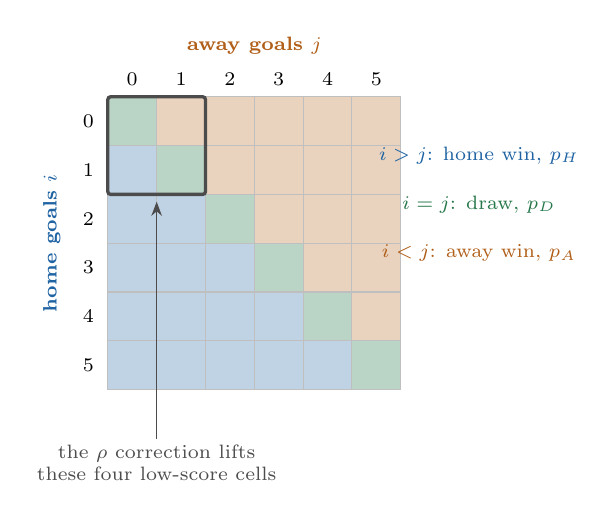
\begin{tikzpicture}[scale=0.62]
\foreach \i in {0,...,5}{
  \foreach \j in {0,...,5}{
    \pgfmathparse{\i>\j ? "blind!28" : (\i<\j ? "market!28" : "joint!32")}
    \edef\col{\pgfmathresult}
    \draw[fill=\col,draw=black!25] (\j,-\i) rectangle ++(1,-1);
  }
}
\foreach \j in {0,...,5}{\node[font=\scriptsize] at (\j+0.5,0.35) {\j};}
\foreach \i in {0,...,5}{\node[font=\scriptsize] at (-0.4,-\i-0.5) {\i};}
\node[font=\scriptsize\bfseries,market] at (3,1.05) {away goals $j$};
\node[font=\scriptsize\bfseries,blind,rotate=90] at (-1.15,-3) {home goals $i$};
\node[font=\scriptsize,blind] at (7.6,-1.2) {$i>j$: home win, $p_H$};
\node[font=\scriptsize,joint] at (7.6,-2.2) {$i=j$: draw, $p_D$};
\node[font=\scriptsize,market] at (7.6,-3.2) {$i<j$: away win, $p_A$};
\draw[very thick,black!70,rounded corners=1pt] (0,0) rectangle (2,-2);
\node[font=\scriptsize,black!70,align=center] at (1,-7.5) {the $\rho$ correction lifts\\these four low-score cells};
\draw[black!70,-{Stealth[length=1.8mm]}] (1,-7.0) -- (1,-2.15);
\end{tikzpicture}
\end{center}

Real football produces more 0--0 and 1--1 draws than two independent Poissons
predict, because teams shut games down. That is what $\rho$ repairs, and it is
fitted separately for each league on held-out matches.

\section*{The market, and the blend}

Odds are payout multipliers. Their reciprocals are implied probabilities, and
they sum to more than one: that excess is the bookmaker's margin. Removing it
gives $\pi$.

\[
\underbrace{\tfrac{1}{2.10}+\tfrac{1}{3.50}+\tfrac{1}{3.80}}_{\textstyle 1.025}
\;\longrightarrow\;
\pi=(0.464,\ 0.279,\ 0.257)
\]

The blend is a weighted geometric average, done in log-odds space so that it
pulls hardest on the extreme probabilities --- which is exactly where the
model's error is largest:
\[
\hat p_k \;\propto\; \pi_k^{\,1-w}\; p_k^{\,w},
\qquad k \in \{H,D,A\}
\]

\begin{center}
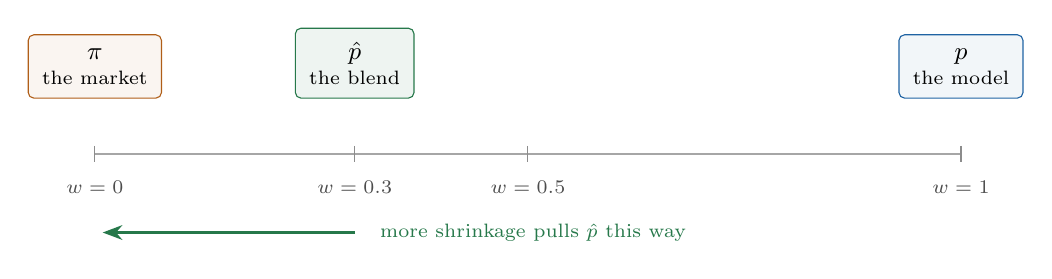
\begin{tikzpicture}[scale=1]
\draw[thick,draw=black!35] (0,0) -- (11,0);
\foreach \x/\lab in {0/{$w=0$},3.3/{$w=0.3$},5.5/{$w=0.5$},11/{$w=1$}}{
  \draw[black!45] (\x,0.1) -- (\x,-0.1);
  \node[font=\scriptsize,black!70] at (\x,-0.42) {\lab};
}
\node[marketbox,anchor=south] at (0,0.7) {$\pi$\\[-2pt]\scriptsize the market};
\node[blindbox,anchor=south] at (11,0.7) {$p$\\[-2pt]\scriptsize the model};
\node[jointbox,anchor=south] at (3.3,0.7) {$\hat p$\\[-2pt]\scriptsize the blend};
\draw[flow,draw=joint] (3.3,-1.0) -- (0.1,-1.0);
\node[font=\scriptsize,joint,anchor=west] at (3.5,-1.0) {more shrinkage pulls $\hat p$ this way};
\end{tikzpicture}
\end{center}

$w$ is fitted on out-of-fold predictions over every earlier season, by whichever
value predicts held-out results best. We fitted it two further ways as a check:
using only the matches we would actually bet, and with a different formula that
shrinks the gap evenly rather than in log-odds. All three agreed.

\newpage
\section*{One match, traced end to end}

\begin{center}
\begin{tabular}{@{}rllp{6.4cm}@{}}
\toprule
& \textbf{Symbol} & \textbf{Value} & \textbf{What happened}\\
\midrule
1 & $x$ & 66 numbers & Elo 1712 vs 1655, home side averaging 1.7 goals
                       over five. No price anywhere in here.\\[2pt]
2 & $\lambda_H,\lambda_A$ & $1.62,\ 1.14$ & Stage 1's view of how the match
                       will be played.\\[2pt]
3 & $p$ & $(0.49,\ 0.25,\ 0.26)$ & The scoreline grid summed into three
                       regions.\\[2pt]
4 & $o$ & $(2.10,\ 3.50,\ 3.80)$ & Closing average odds; reciprocals sum to
                       1.025.\\[2pt]
5 & $\pi$ & $(0.464,\ 0.279,\ 0.257)$ & The same prices with the 2.5\% margin
                       removed.\\[2pt]
6 & $\hat p$ & $(0.472,\ 0.270,\ 0.258)$ & Blended at $w=0.3$. The model moved
                       the home probability by less than a point.\\[2pt]
7 & $e$ & $(+0.008,\ -0.009,\ +0.001)$ & The edge on each outcome.\\[2pt]
8 & $\tau$ & $0.021$ & Read off earlier seasons. The best edge here is 0.008,
                       well under it.\\[2pt]
9 & --- & \textbf{no bet} & The normal outcome. We act on about one match in
                       seven and abstain on the rest.\\
\bottomrule
\end{tabular}
\end{center}

\section*{What actually happened}

In every one of the five test seasons, the fitted weight came out
\[
w = 0.
\]
Put that into the blend and it collapses: $\hat p = \pi$, every edge in step~7
is exactly zero, and the corrected model \emph{is} the market price.

That is not a bug and it is not a broken optimiser --- we swept $w$ by hand and
every step away from zero makes the predictions worse. It is a finding. Stage~1
scores 1.0145 in log loss against the market's 0.9950, where knowing nothing
scores 1.0770. The model closes about three quarters of the distance from
ignorance to the closing price, and still adds nothing the price does not
already contain.

The mechanism itself works. With no shrinkage the model expects a 127\% return
on the bets it selects and earns 2\%; with full shrinkage it expects 10.8\% and
earns 6.2\%. That collapse, from a 125-point gap to a 5-point one, is the
winner's curse being removed exactly as the theory predicts. What the data
denies us is anything to correct.

\end{document}
